\section{Background}


The University of Illinois at Urbana-Champaign is an ideal model system for
this work because of its diverse energy mix. Previous work
characterized this energy grid and optimized the size of a nuclear reactor
for decarbonization \cite{dotson_optimal_2020}. Due to the degree of wind
penetration, the University is sometimes
forced to sell electricity back to the grid operator, MISO, at a loss because
of overproduction
from wind energy. Thus, a reliable prediction of electricity production from
wind and other variable sources will reduce the likelihood of these events.
Figure \ref{figure:vre} shows the total demand and net demand profiles at the
\gls{uiuc}.
Daily variations in electricity demand are reasonably predictable, with a
usual evening minimum around 40MW. Weekdays have peaks near 50MW and are
distinguishable from weekends with peaks near 45MW. When renewable energy is
included in the mix, regular changes from day/night and weekday/weekend are
impossible to track by inspection. This lack of predictability is primarily due
to renewables' tight coupling with chaotic weather systems. The chaotic nature
of weather, and by extension renewable energy, indicates that there are
dynamics that can be learned even without a physical model.
\begin{figure}[h]
  \centering
  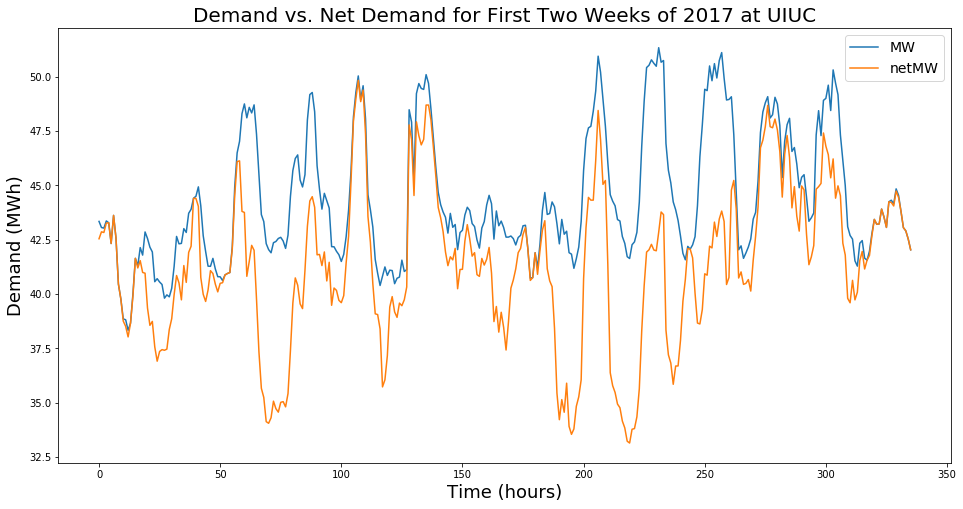
\includegraphics[width=\columnwidth]{renewable_variability}
  \caption{Comparison between total demand and demand accounting for renewable
   energy. ``netMW'' is the total minus wind and solar.}
  \label{figure:vre}
\end{figure}

\glspl{ESN}, a flavor of reservoir computing, are a modern
machine learning algorithm that can learn the dynamics of a chaotic system.
Pathak et. al used an \gls{ESN} to predict the
evolution of a laminar flame front up to seven Lyapunov
times in the future \cite{pathak_model-free_2018, wikner_combining_2020}. A
Lyapunov time simply measures the timescale at which chaos makes initial
predictions useless. The effect of chaos typically overwhelms conventional
predictions after a single Lyapunov time, by definition.
The Lyapunov time for a weather system is on the order of a few days but
depends on the regional environment. \glspl{ESN} have also been used to
forecast multivariate time series \cite{bianchi_reservoir_2020}. \glspl{ESN}
are unique among neural
networks in their ease of implementation and training speed. This is owed to its
sparse network architecture \cite{pathak_model-free_2018,
wikner_combining_2020, vannitsem_predictability_2017}. However,
their simplicity is balanced by the need for carefully chosen hyperparameters
for the desired task \cite{lukosevicius_practical_2012}.
Accurate renewable energy forecasts with \glspl{ESN} could enable new load
following strategies for nuclear power plants.
